%%% Realisering for optimering af gate-modstand %%%


\subsection{Switch-tid}
Implementeringen af den optimerede switch-tid testes ved, at måle MOSFET'ens gate signal. Det signal er vist på figur~\ref{fig:realisering_switch_tid_3}, hvor kanal 1 er current-sense signalet, som giver et billede af MOSFET'ens strøm, og kanal 2 er MOSFET'ens gate. Her aflæses switch-tiden til ca. $40ns$. Det kan dog ses der fremstår to plateauer på gate-signalet, hvilket ikke kan forklares. Det vurderes dog, at det andet plateau ikke vil have indflydelse på tabet i MOSFET'en, da strømmen er mindre end 0 på det pågældende tidspunkt.

Derudover kan peak-spændingen over MOSFET'en aflæses på figur~\ref{fig:realisering_switch_tid_drain_3} til ca. $90V$.hvilket er med en margin på $40\percent$ til dens breakdown spænding. Resultaterne for analysen, simuleringen og realiseringen indføres i tabel~\ref{tab:resultat_switch_tid_3}. Her er simuleringen dog foretaget med en anden MOSFET.

\begin{table}[H] 			
	\centering
	\begin{tabularx}{\textwidth}{|X|c|c|c|}
		\hline
		\textbf{Tid} & \multicolumn{3}{|c|}{\textbf{Resultater}} 										\\ \hline
		& A & S & R 									\\ \hline
		$T_{ch}$    & $37.2ns$ & $29.4ns$ & $40ns$ 											\\ \hline 
		$V_{ds,pk}$ &          & $110V$   & $90V$		\\ \hline 
		
	\end{tabularx}
	\caption{Resultater for analyse, simulering og realisering af switch-tid}
	\label{tab:resultat_switch_tid_3}
\end{table}

\begin{figure}[H]
	\center
	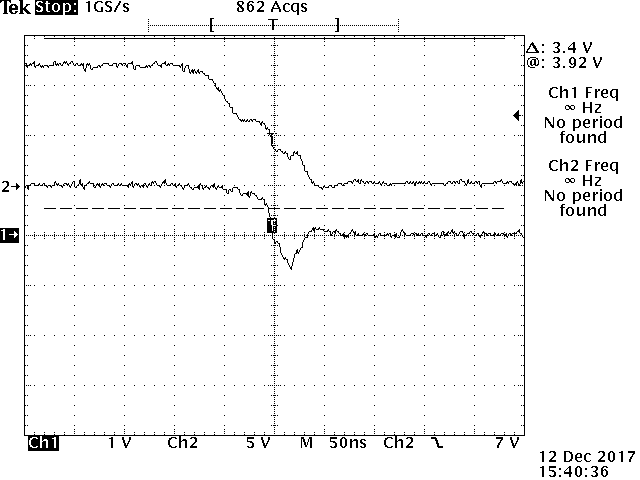
\includegraphics[max width=0.7\linewidth]{/tex/3iteration/billeder/Realisering/Gate_vs_cs.png}
	\caption{Realisering af switch-tid for MOSFET - 3. iteration}
	\label{fig:realisering_switch_tid_3}
\end{figure}

\begin{figure}[H]
	\center
	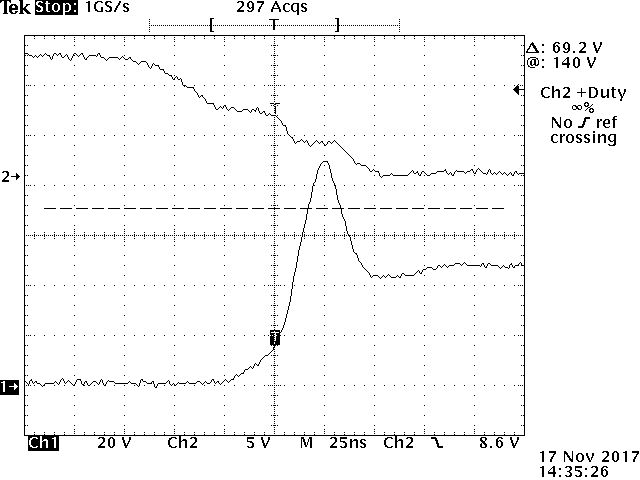
\includegraphics[max width=0.7\linewidth]{/tex/3iteration/billeder/Realisering/Realisering_switch_tid.png}
	\caption{Realisering af switch-tid for MOSFET - 3. iteration}
	\label{fig:realisering_switch_tid_drain_3}
\end{figure}